%%%%%%%%%%%%%%%%%%%%%%%%%%%%%%%%%%%%%%%%%%%%%%%%%%%%%%
\section{BlueBridge Design}
\label{sec:overview}
%%%%%%%%%%%%%%%%%%%%%%%%%%%%%%%%%%%%%%%%%%%%%%%%%%%%%%
In the following section, we outline our design approach of the BlueBridge shared memory system. This roadmap is by no means final and will be subject to change and amendments during realization. Scope as well as generalizability of the system are not yet determined, and may vary to accommodate particular application types. 
Our assumptions about network and eventual switch configuration capabilities are drawn from the OpenFlow Switch specification v1.50~\cite{ONF_Switch} and the P4 programmable switch paradigm~\cite{p4}.

\subsection{Assumptions}

As BlueBridge is intended to run in constrained and controlled datacenter environments we make several assumptions about the environment and underlying technology of the project.

Communication in a distributed shared memory system should be inexpensive and performant. Ideally, a remote operation provides a substantial advantage over disk-reads and the penalty compared to a local memory access is minimal.
As a consequence, we expect a working prototype to be able to support RDMA over Converged Ethernet (RoCEv2) as transmission protocol for our remote paging requests to be satisfactory. We are confident in these assumptions, as recent research has demonstrated the potential of this comparably modern technology.~\cite{commodityrdma}

Second, we require our system to run in a reliable network environment with state-of-the-art network components. We assume that link-speed as well as switch capabilities are sufficient to handle the communication load of the distributed system. We do not take packet loss into consideration and expect reliable transmission from each node.

Third, we currently do not intend to scale beyond a 42-U rack size managed by a single ToR switch. Every rack is an autonomous cluster computationally independent of other entities in the network. Furthermore, any packet exchange between nodes in the cluster will only requires a single hop over the managing switch. For our current approach we also disregard extensive replication and high fault-tolerance techniques. As a single point-of-failure, a malfunctioning switch or controller will imply a total system failure.

\subsection{Proposed Design Overview}
% \subsubsection{Virtual Memory System}
The eventual design goal of BlueBridge is to implement a software-based virtual memory system in conjunction with a distributed memory platform. The approach is founded upon a partitioned global address space (PGAS), 4096 bytes page implementation.
\begin{figure}[t]
    \centering
    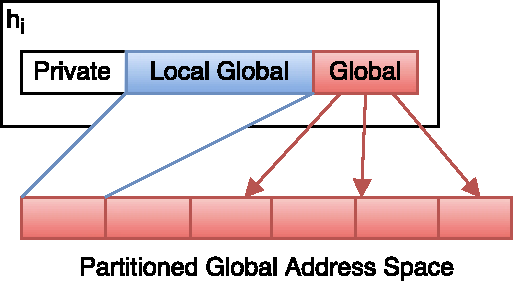
\includegraphics[width=\columnwidth]{Images/BlueBridgeHostMemory.pdf}
    \caption{Illustrations of how global memory is stored in a BlueBridge host.}
    \label{fig:pgas}
\end{figure}
Each machine's memory section contains a private and a global address space (see Figure \ref{fig:pgas}). Private memory is only accessible to critical or privileged processes of the local host, it is not shared with any other node. Global address space is divided into a local and remote section, the former residing physically on the machine.
Local global memory encompasses the address space a server provides for other machines to use, it may also contain memory the host has fetched from remote machines and stored for computation. The global address space is comprised of a collection of pointers the local machine has either reserved from remote hosts or requested for future operations.
% \ugh{All remote memory addresses are mapped locally using the \texttt{mmap()} call and accessed on demand} \hl{needs to be verified}. 
In order to preserve locality, hosts are aware of the global memory available on the machine and all operations are performed locally. In case of a remote fetch, data is written back to the original host. In a scenario involving disaggregated memory and servers acting as memory banks, remote memory will treated as a single uniform address space.
% \subsubsection{The Blueprint}
BlueBridge follows a simple design concept, as shown in Figure \ref{fig:blueprint}.

\begin{figure}[t]
    \centering
    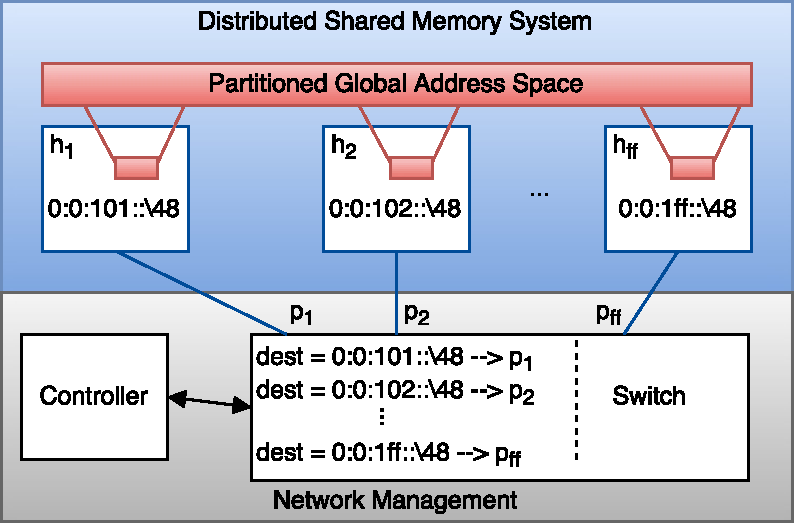
\includegraphics[width=\columnwidth]{Images/BlueBridgeMemory.pdf}
    \caption{High-level blueprint of BlueBridge architecture.}
    \label{fig:blueprint}
\end{figure}

The core of the proposal is a divergence of conventional memory address properties. BlueBridge does not rely on typical PGAS memory design and directly encodes memory addresses as IPv6 pointers. Each client acquires remote memory in the form a 128 bit IPv6-conform address. Instead of storing a request in the payload of a network packet, any subsequent request will be directly inserted into the destination header of the packet.
This design choice allows for powerful operations in the network space which may greatly simplify consistency and coherence management in a DSM system. Any request or operation can be routed, forwarded, copied, or modified directly without hosts being required to track state. Both receiver and sender remain fully unaware of the remote location or current state of the memory as these operations are handled by dynamic network functions.

To support the architectural concept we utilize a software-defined switch as well as controller handling all required operations. To avoid overloading the switch, entries are kept minimal. Servers are assigned a subnet range which represents a global memory partition. In combination with the pointer address, this subnet range creates an unique identifier in the packet header. 

If a client performs an operation requiring the use of a remote pointer, it will insert the stored pointer into the destination IP field of the IPv6 header and send the packet. Since the header contains the unique node ID, the switch is able to instantaneously forward the packet to the correct port. The server will extract the pointer and specific command out of the destination header, perform the specified operation, and reply to the source IP of the packet (which is the unique ID of the client). A client ``keeps track" of an address by extracting the source ID identifier of the replying owner.
Neither server nor client are required to store any information about the location of other machines. For $n$ servers the switch only has to maintain $n$ basic routing entries, mapping each subnet to a specific port.
\newcommand\ipsample{{"0","0","0","0","0","0","0","0","0","1","0","3","0","3","0","0","d","0","8","4","9","5","0","1","0","0","0","0","0","0","0","0"}}

\begin{figure*}
\hspace*{-10px}
  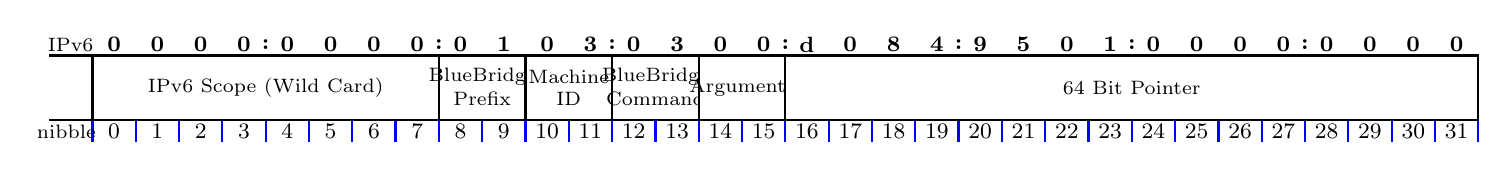
\begin{tikzpicture}[scale=0.55]
    \foreach \x in {0,...,31}
		\node at (\x+0.5,0.25) {\footnotesize \x};
	\foreach \x in {0,...,32}
    \draw[thick, blue] (\x,0) -- (\x,0.5);
    \node[thick] (bit1) at (-0.6,0.24) {\scriptsize nibble};
	\draw [thick] (-1, 0.5) -- (-0,0.5);

    \node[thick] (bit1) at (-0.5,2.25) {\scriptsize IPv6};
	\draw [thick] (-1, 2) -- (-0,2);

	\filldraw[thick,draw=black, fill=white] (0,0.5) rectangle (8,2);
	    \node (mode) at (4,1.25) {\scriptsize IPv6 Scope (Wild Card)};
	\filldraw[thick,draw=black, fill=white] (8,0.5) rectangle (10,2); 
	    \node (mode) at (9,1.5) {\scriptsize BlueBridge};
        \node (mode) at (9,1) {\scriptsize Prefix};
	\filldraw[thick,draw=black, fill=white] (10,0.5) rectangle (12,2);
	\node (mode) at (11,1.5) {\scriptsize Machine};
	\node (mode) at (11,1) {\scriptsize ID};
	\filldraw[thick,draw=black, fill=white] (12,0.5) rectangle (14,2);
	    \node (mode) at (13,1.5) {\scriptsize BlueBridge};
	    \node (mode) at (13,1) {\scriptsize Command};
	\filldraw[thick,draw=black, fill=white] (14,0.5) rectangle (16,2);
	    \node (mode) at (15,1.25) {\scriptsize Arguments};
	\filldraw[thick,draw=black, fill=white] (16,0.5) rectangle (32,2);
	    \node (mode) at (24,1.25) {\scriptsize 64 Bit Pointer};

	%\filldraw[thick,draw=black, fill=white] (0,2) rectangle (32,2.5);
	\foreach \x in {4,8,12,16,20,24,28}
	    \node at (\x,2.25) {\footnotesize \textbf{:}}; 

	\foreach \x in {0,...,31}
        \node at (\x+0.5,2.25) {\footnotesize \textbf{{\pgfmathparse{\ipsample[\x]}\pgfmathresult}}};
\end{tikzpicture}
\caption{The IP destination structure. The top row represents a sample IPv6 
request which is mapped to the structure below.}
\label{fig:ipv6}
\end{figure*}

\subsection{Operations}

The client library currently consists of simple CREATE, READ, UPDATE, DELETE (CRUD) functions for a higher-level application to utilise. The current operational plan for each procedure is as follows:

\paragraph{\textbf{CREATE}}
If a client needs to allocate or reserve a remote memory section, it will call CREATE. The function selects a random ID of the available server range and sends a IP packet containing the create command and destination ID. The switch forwards the packet to the corresponding server. After allocation of a local pointer has been successful on the server side, it stores the address in the payload of the packet and responds with an ACK message. The client will extract the pointer as well as the unique identifier of the server, merge the structure into a unique global pointer, and store it for future use.

The size of a single allocate operation is limited to 4096 byte pages. It may be beneficial to allow clients the specification of arbitrary allocation size. If the size exceeds a certain threshold, both parties can switch to a TCP connection for more efficient data transfer.

For future work, we are considering to render clients fully agnostic of the destination and introduce load-balancing capabilities on the switch. Clients will send generic CREATE destination requests, which will be distributed by the software switch based on optimal locality or load. This approach is possible as the switch is able to forward the generic packet to a controller, which could decide the current optimal placement. It remains to be seen if the trade-off between additional request latency and efficient placement will provide long-term gains.

We are also considering the use of broadcast allocation to inform all other clients of a newly available memory address. Information about the location of shared variables can thus be quickly spread through the network.

\paragraph{\textbf{WRITE}}
Once a client has acquired a pointer, it is able to write to the remote address by inserting the IPv6 structure into the packet header and coupling it with an WRITE command. Data that is to be written is encapsulated in the payload. The server will extract the pointer, store the data of the payload in its global address space, and acknowledge to the client that the operation has been successful. We are currently intending to support three different types of write commands natively.
\begin{itemize}
    \item \textit{Allocate Writes.}
    The client will insert a ALLOCATE-WRITE command in the header as well as the data content in the payload. The server will write the data to its local memory and provide the allocated memory address to the client.
    \item \textit{Blind Writes.}
    Blind writes are simple asynchronous operations unaware of any consistency or coherence semantics. The content of a blind-write packet is directly written to the server disregarding any that has been previously stored in the block. Applications may use this type of write at their own risk.
    \item \textit{Updates.}
    Updates are transactional procedures which guarantee data consistency and correctness. An update operation requires a READ before being able to write data. Update operations transfer ownership temporarily to the accessing node. Further semantics are described in the READ section.
\end{itemize}

\paragraph{\textbf{READ}}
A READ operation is functionally similar to the WRITE call. The server will extract the pointer, store the memory content in the payload, and send the data to the client.

In a concurrent and asynchronous implementation involving direct memory access it may occur that an other client has fetched the same memory and is currently modifying the data block. Our approach to solve this potential race condition is as follows:

As soon as a client has requested an UPDATE operation on a particular memory address, the switch will install a temporary redirect route forwarding all subsequent requests to the current owner of the memory section. The new owner may either reject or process the requesting, depending on the consistency policy of the system or application. To prevent stale reads before the redirect is updated, the server will invalidate its memory section until the client has rewritten the data. After a successful procedure, all temporary flows are removed and data exchange continuous as usual.

\paragraph{\textbf{DELETE}}
A DELETE operation is a simple \texttt{free} or \texttt{memset(0)} operation on the server side depending on desired outcome. If the memory is to be re-used, it can be set to zero, if it is supposed to be deallocated, it can be freed. The client can call DELETE at any time. To prevent the remaining machines from using a stale pointer we are planning to utilise a broadcast message containing the memory address in question. The switch forwards the message to all machines in the network and any affected client will invalidate its pointer.


All of these operations are are stored in the IPv6 header of the packet encoded as single byte, providing a total of 127 unique commands. Storing commands in the header also allows the central coordinating switch to reroute or reject packets based on the nature of the request without involving a server. This feature also opens up the possibility of the control plane to monitor the computational state of the system and interject if necessary.

\subsection{Control Plane}
As the majority of management and coordination operation are shifted into the network, the controller as well as the software switch have to be able to bear a significant amount of computation and load.
The amount of network nodes a packet traverses until its destination has to be minimal. Avoiding a flow table "cache miss" is desired as much as possible is desired as flow-table updates are expensive. These aspects require a proactive flow-installation system and the controller to have global knowledge of the memory layout. Flow table entries in the switch need to cover most common events.
% \paragraph{\textbf{Routing}}
In the default case, the controller will monitor active nodes in the system and proactively install corresponding flow entries. Any packet that matches a particular IPv6 CIDR address will be forwarded to the owner without any further overhead.
\paragraph{\textbf{Update operations}}
\label{par:updates}
Update operations require consistency which can be enforced by the control plane. For any header containing an UPDATE command, the switch will forward the packet to the node as well as the controller to process.
The packet will trigger the controller to call a flow-table update procedure which will install a redirect entry of the specific pointer address to the new owner.
In order to mitigate the exhaustion of flow tables, these entries must be temporary.
After installing the flow rule, two possible events may occur. Either the client writes the content back to the original
node and triggers a new controller action to delete the entry, or the flow expires. If a flow expires, the controller as well as server assume that the client operation has failed and the memory section is marked available again. The delayed write operation of the client will be rejected. 


\paragraph{\textbf{Monitoring}}
Port mirroring of switch traffic as well as out-of-band monitoring and management of client machines allow for a comprehensive central view of the controller of all network events. Opportunities may include fast-failover in case of single machine failure, or identification and dynamic rebalancing of hot memory partitions.

In addition to conventional strategies, a realizable migration concept may include live-updating of flow entries to move traffic to less active nodes. As the switch is able to route by inspecting commands in the destination header, it is possible to redirect WRITE operations to a different host. After successful completion, the controller will install a permanent flow entry redirecting requests to the new owner.
A client thus incidentally and seamlessly migrates data while keeping the data flow of the system intact.
One significant drawback of this method is the eventual fragmentation and subsequent switch table exhaustion. 
Consequently, we intend to assess and thoroughly evaluate the feasibility and computational complexity of specific procedures leveraging these two properties.

\paragraph{\textbf{Controller performance and flexibility}}
The control plane is a crucial component of the BlueBridge system. As it primarily rests upon the underlying controller architecture, we require a mature, efficient, and reliable framework.
Potential candidates under investigation include Beacon, Nettle, OpenDaylight, and ONOS. While ONOS~\cite{onos} and OpenDaylight~\cite{odl} are comprehensive frameworks with a multitude of features and industry support, they are comparably slow.~\cite{controller_perf1} Beacon~\cite{beacon} and the Nettle language~\cite{controller_perf2} feature extremely fast processing and response times, but are largely academic. Beacon is not under active development and Nettle is written in Haskell with unclear maturity and flexibility. 
BlueBridge is tightly coupled to the capabilities of the control platform and we have to weigh benefits of each control plane paradigm. Opting for the right framework is essential for the system to succeed.

% \subsection{Discussion}
% Although BlueBridge is still in the prototyping stage, particular limitations and properties of the design may be fundamental.

% \subsubsection{Switch and Controller Performance}
% It is unclear, if hardware switches and control software are capable of handling the update frequency demanded by the current design.
% Complex operations such as migration or updates may quickly exceed maximum switch performance and flow table efficiency. Evidence suggests that software switch tables are easily exhausted under heavy load.~\cite{controller_perf1,controller_perf3}
% If and only if the flow table size, updates,  and expiration times are kept sufficiently small, we can expect the system to remain stable.
% \subsubsection{Managing a Dynamic Address Space}
% Migrating and splitting memory partitions of the global address space introduces substantial complexity. In our design, a memory address is a unique heap pointer exclusive and only correct on the machine it has been allocated in. A redirected client access as described in section \ref{par:updates} will lead to incorrect access or corruption on a different machine. Maintaining a specific mapping on either the client or server side is costly and violates the agnostic end-host principle of BlueBridge. A potential solution is to notify the client to update its allocated memory address using either over broadcasts or specific controller messages. The client will update its mapping with the pointer and source address of the new owner, preserving correctness in the system.

% \subsubsection{Designing for failure tolerance and scalability}
% BlueBridge is built around one single switch maintaining all flow tables on rack-scale, interacting with a single controller. It is an open question to what level the system should be fault-tolerant, if at all. While it is feasible to mirror the controller as well as the switch without incurring too much overhead, it may be costly. Failure-tolerance may be pushed to applications to reduce configuration and operational complexity.